
\def\risp#1#2{\centerline{{\small\bfseries Рис.\ \the\zagn.#1 .}\ {\small #2}}}
\def\tabp#1#2{\noindent{\small\bfseries Таблица\ \the\zagn.#1 .}\ {\small #2}}
\def\eqn#1{(\the\zagn.#1)}
\def\noq{\global\advance\numq by 1\eqno(\the\zagn.\the\numq)}

\zag{Экспериментальные методы}

\subzag{Экспериментальные методы исследования интегральной
интенсивности и спектрального состава рассеянного света}
\thispagestyle{empty}

\vskip 5mm
\markboth{\hfill\small Экспериментальные методы исследования интегральной
интенсивности\hfill}{}

Современное состояние теории жидкостей не позволяет вычислить
величину абсолютной интенсивности светорассеяния в чистых
жидкостях, а расчет по термодинамической теории наталкивается на
ряд трудностей. Экспериментальное определение рассеивающей
способности чистых жидкостей поэтому очень важно для дальнейшего
развития теории рассеяния света в жидкостях.

Точное знаник абсолютной интенсивности светорассеяния жидкостей,
помимо теоретического, представляет большой практический интерес
с тех пор, как предложенный Дебаем в 1944 году \ метод
определения молекулярных весов полимеров по рассеянию света в
растворах стал одним из самых точных и удобных методов. Однако
для конкретной интерпретации полученных результатов этот метод
требует не только точного значения рассеивающей способности
эталонной жидкости, используемой для калибровки прибора, но также
уточнения физического смысла значения $\left({n-n_0\over
c}\right)$. В теории Дебая используется макроскопическое значение
этой величины, в то впремя как строгая теория молекулярного
рассеяния предполагает флуктуационное значение производной
${\partial(n-n_0)\over\partial c}$. Здесь $n$ и $n_0$ ---
показатели преломления раствора и растворителя соответственно, а
$c$ --- концентрация раствора.

До 1948 года результаты многочисленных исследований разных
авторов находились в хорошем согласии между собой. Это были
экскпериментальные исследования фотометристов французской школы
Кабанна, известной своими работами по рассеянию света в
жидкостях, начиная с работы Мартина и Лермана в 1922 году .
Измерения, в основном, были фотографическими, при которых
сравнивались яркости рассеянного и падающего пучков.

После того, как метод Дебая определения молекулярных весов
полимеров по рассеянию света начал получать широкое применение
ввиду его простоты. Оказалось, что результаты этого метода не
согласуются с результатами других методов определения
молекулярных весов полимеров. Согласие было бы только в том
случае, если бы коэффициент рассеяния $R$ жидкости, используемой
в качестве эталона, был бы на 30\% выше.

Мы остановимся подробно на фотоэлектрических измерениях Карра и
Зимма , так как эти авторы первыми выступили против <<
низких>>\ значений для константы рассеяния бензола, и
последующие  исследователи, применяя подобный фотоэлектрический
метод, ссылаются на эту работу, как на основное исследование по
определению абсолютной рассеивающей способности бензола. Карр и
Зимм определяли мутности растворов полистирола в бутаноне и
дихлорэтане. По известным мутностям, пользуясь соотношением,
авторы расчитывают $R_{90}$ раствора. Затемпроводятся
относительные измерения интенсивности света, рассеянного бензолом
и ${\rm CCl_4}$ под углом 90$^{\circ}$. к падающему пучку по
сравнению с интенсивностью света, рассеянного раствором полимера.

Мутности $\tau$ растворов полистирола были определены тремя
методами. Так как аналогичные методы применяются и в работах
других авторов, рассмотрим их подробно.

Первый метод заключается в сравнении интенсивности света,
рассеянного раствором в направлении 90$^{\circ}$ к падающему
пучку, с интенсивностью падающего пучка. Сравниваемые световые
потоки в этом случае отличаются в $10^{6}$ раз, и прямое
сравнение их затруднительно.

Для ослабления падающего потока приходится вводить серые фильтры
большой плотности. Для того, чтобы исключить все пространственные
измерения, кроме глубины рассеивающего объема и сделать подобными
условия регистрации сравниваемых световых пучков, поступают
следующим образом: сравнивают светорассеяние растворов с
рассеянием стандартных диффузоров с известными отражательными
свойствами. В качестве диффузоров использовались фарфоровые
пластинки, покрытые MgO и $\rm MgCO_3$. Предполагалось, что
диффузоры << идеальные >>, т. е. распределение интенсивности
света в пространстве подчиняется косинусному закону Ламберта.

На рис. 5.1 представлена схема установки. Источник, ртутная
лампа, фокусируется на диафрагму D, расположенную в фокальной
плоскости линзы L, посылающей параллельный пучок на кювету
рассеяния. Приемником служит фотоумножитель PM с входным
отверстием A, за которым расположена система подвижных линз R ---
S, позволяющая получать на катоде фотоумножителя постоянное по
размерам изображение диафрагмы A.

\begin{figure}[tbp]
\centerline{\hbox{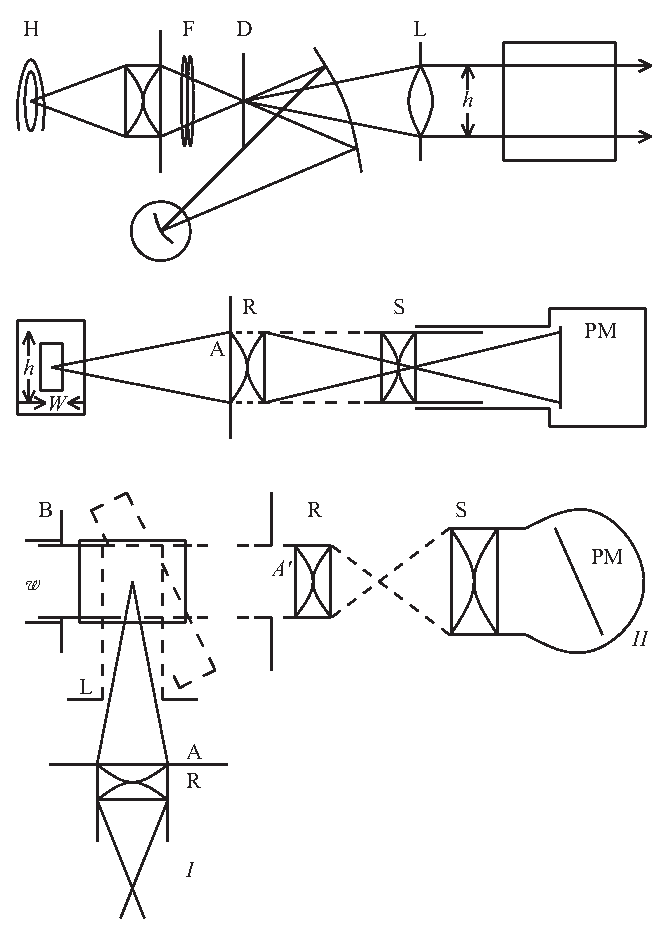
\includegraphics[scale=1.0]{Ris/ris_eps/ris5_1.eps}}}

\risp{1}{Методы Карра и Зимма}
\end{figure}

В положении II, если площадь отверстия диафрагмы, которая
определяет пространство наблюдаемого пучка равна $A'$, фотометр
примет поток
$$F_1=I_0A't_1,\noq$$
где $I_0$ --- интенсивность падающего света, $t_1$ --- ослабление
ее нейтральными серыми фильтрами.

В положении I, если площадь отверстия ограничивающей диафрагмы,
расположенной на расстоянии $r$ от рассеивающего объема, равна
$A$, рассянный поток, получемый фотометром
$$F_5=i_{90}\cdot A={3\over16\pi}\tau{I_0[hw\cdot l]\over
r^2}A,\noq$$
где $h,\ w$ и $l$ определяют размеры рассеивающего объема.
Отношением ${F_5\over F_1}$ определяется искомая мутность
раствора
$$\tau={16\pi\over3}\left({F_5\over F_1}\right){r^2\over[hw\cdot
l]}\cdot{A\over A'}t_1.\noq$$
Если освещенность падающего света $I_0$ и диффузор помещается
вместо рассеивающей кюветы под углом 45$^{\circ}$ к падающему
пучку, то световой поток, падающий на единицу поверхности
диффузора $I_0\cos\alpha$, а светимость поверхности диффузора
$S=I_0\cos\alpha r_f$, где $r_f$ --- коэффициент отражения <<
идеального>>\ диффузора. Для источников, подчиняющихся закону
Ламберта:
$$S=\pi\cdot B,\hskip 4mm B\cdot\sigma=I,\noq$$
где $B$ --- яркость поверхности диффузора; $\sigma$ --- площадь
поверхности; $I$ --- сила света, испускаемого диффузором.
Освещенность отверстия фотометра, расположенного на расстоянии
$r$ от диффузора
$$E={I\over r^2}={Bhw\over r_2},$$
и полный поток, получаемый фотометром в положении I, когда кювета
с раствором заменена диффузором
$$F_6=E\cdot A={I_0\cos\alpha r_f[h\cdot w]\over\pi r^2}At_2,\noq$$
где $t_2$ --- частичное ослабление падающего света, необходимое
для сравнения $F_5$ и $F_6$.
Таким образом, для определения $\tau$ необходимо сделать два
измерения $F_5$ и $F_6$. Окончательно
$$\tau={16\over3l}\cdot{\sqrt{2}\over2}r_ft_2\left({F_5\over
F_6}\right).\noq$$

Для ослабления падающего пучка использовались жидкие фильтры.
Каждый фильтр поглощал 27\% проходящего света. Калибровка
фильтров производилась на той же установке с диффузором.
Ослабление определялось как отношение двух показаний фотометра,
когда фильтр находился на пути светового пучка и вне его.
Коэффициент $r_f$ для диффузора рассчитывался теоретически из
данных по полному отражению поверхностей MgO и  MgCO$_3$, и,
кроме того, определялся экспериментально.
Следует отметить, что если для светящихся поверхностей закон
Ламберта строго не выполняется, то интенсивность света,
рассеянного под углом $45^{\circ}$ может отличаться от
интенсивности вычисленной согласно косинусному закону из данных
по полному отражению поверхности.

Исследования, посвященные изучению рассеивающей способности
поверхности MgO и MgCO$_3$, показали, что даже при самом
тщательном приготовлении диффузоров наблюдаются отклонения их от
<< идеальных>>\ .
С другой стороны, невыполнение точного угла при установке
диффузора приведет к значительной экспериментальной ошибке в
определении интенсвиности падающего пучка. Метод поперечного
рассеяния дает величину $\tau$, которая нуждается в ряде
исправлений:

1. Авторы вводят поправку $C_{\rho}$, обусловленную б\'ольшей
чувствительностью фотоумножителя к горизонтально-поляризованному
свету, чем к вертикально поляризованному свету.
Карр и Зимм оценивают это различие как 7-12\%, в зависимости от
размера изображения на поверхности фотокатода. Таким образом,
очень важно в данном эксперименте, чтобы размеры светового пятна
на катоде оставались постоянными при переходе от измерений с
раствором, к измерениям с диффузором.
Из-за различной геометрии пучков в этих двух случаях, постоянство
это не всегда достигается передвижением проектирующих линз.
Отсутствие специального контроля за размерами светового пятна на
катоде также может служить источником ошибок.

2. Поправка, которую Карр и Зимм вводят на расходимость лучей,
выходящих из кюветы рассеяния, вследствие различия показателей
преломления, легко может быть понята из рассмотрения рис. 5.2.
Рассматривается случай прямоугольной кюветы, на которую падает
параллельный пучок света.
Действительный поток света, который собирается фотоумножителем,
содержится не в телеснов угле $\theta_1$, а в угле $\theta_2$.
Поправка учитывается следующим образом
$$C_n=\left({\theta_2\over\theta_1}\right)^2=n^2\left[1-{b(n-1)\over
r\cdot n}\right]^2,\noq$$
где $b$ --- расстояние от центра рассеивающего объема до стенки
кюветы; $r$ --- расстояние от центра рассеивающего объема до
отверстия фотоумножителя A; $n$ --- показатель преломления
рассеивающей среды, заполняющей кювету. Если расстояние от
входного отверстия фотометра много больше величины кюветы $(r\gg
b)$, то $C_n=n^2$. В случае когда фотометр вплотную придвинут к
стенке кюветы, т. е. $r=b$, $C_n\rightarrow 1$.

3. Поправка $C_v$ на действительны объем, наблюдаемый фотометром,
по величине значительно меньше, чем $C_n$. Фотометр << видит>>\
объем несколько больший, чем объем, определяемый размерами $h,\
w$ и $l$ (рис. 5.3). Отверстие фотометра $A=a$ определяет
телесный угол, под которым рассматривается объем $V=l\cdot w\cdot
h$, но элементы $\Delta V$ в добавочном объеме рассматриваются
под телесным углом, который уменьшается при приближении элементов
к наружному краю. Поправка $C_v$ есть отношение количества света,
полученного фотометром от объема $V$, к количеству света,
полученного от действительного объема и выражается следующим
образом:
$$C_v=1-{{b(a+l)\over(r-b)}\over2\left[nl+{b(a+l)\over(r-b)}\right]}.\noq$$
Карр и Зимм считают действительной величину мутности раствора,
полученную путем умножения экспериментального значения на $C_n$,
$C_v$ и $C_{\rho}$.

Метод, связанный с наличием такого большого числа поправок
значительный по величине, вряд ли может считаться точным методом
определения $\tau$. Следует отметить, что хотя теоретический
расчет $C_n$ и $C_v$ в случае прямоугольной кюветы не вызывает
сомнений, в эксперименте поправка $C_n$ может значительно
отличаться от вычисленной, так как трудно правильно учесть
геометрические факторы реальной оптической системы.

Второй метод определения мутности раствора полимера --- метод
интегрирующей сферы. Использовалась гипсовая сфера с внутренним
диаметром 13,5 см, внутренняя поверхность сферы покрыта Zn и
затем MgO. В сфере имелось два отверстия $d=1$ см, одно против
другого, A и B. Третье отверстие C в горизонтальной плоскости,
под углом $90^{\circ}$ к двум первым сделано для фотоумножителя,
который регистрирует освещенность стенки противоположной
отверстию сферы. В выходное отверстие B может вставляться
заслонка из $\rm MgCO_3$. Исследуемый раствор помещался внутрь
сферы в цилиндрической кювете, длиной 2 см и диаметром 1,5 см.
Кювета ставилась на специальную подставку. Падающий поток входит
в сферу через отверстие A. Если закрыть заслонкой отверстие B, то
поток входящий в сферу определится по освещенности поверхности
сферы (показания фотометра $F_3$). Затем удаляют входную заслонку
из B, тогда падающий поток проходит через всю сферу, а
освещенность поверхности сферы будет определяться только потоком
рассеянного находящимся в кювете веществом света. Проводятся два
измерения с закрытым отверстием B.  Первое с кюветой, наполненной
растворителем $(F'_4)$, второе с кюветой, наполненной раствором
$(F''_4)$. Величина $F_4$ определяется как разность
$F_4=F''_4-F'_4$ и характеризует поток, обусловленный только
рассеянием растворенного вещества.

Мутность $\tau$ определяется как
$$\tau={F_4\over F_3\cdot l},\noq$$
где l --- длина кюветы. Падающий поток ослабляется теми же серыми
фильтрами, что и в методе поперечного рассеяния.

Нам представляется, что в таком виде метод интегрирующей сферы не
может служить для точного определения величины мутности. Мы
исходим из следующих соображений. Для измеряемого в данной работе
1\% раствора полистирова в бутаноне мутности имеют следующий
порядок величины :

\hskip 1cm $\tau_{\rm \hbox{бутанона}}=0,5\cdot 10^{-4}\ {\rm \hbox{см}^{-1}}$;

\hskip 1cm $\tau_{\rm \hbox{раствора}}=0,5\cdot 10^{-2}\ {\rm \hbox{см}^{-1}}$.

\noindent
При вертикальном падении светового пучка на двух поверхностях
передней стенки кюветы отразится до 0,1 падающего потока. Так как
сфера имеет и входное и выходное отверстия $d=1$ см, то
отраженный свет может попасть на внутренние края входного
отверстия, а если угол, составленный плоскостью передней стенки
кюветы с направлением падающего пучка хоть на несколько
(2-3$^{\circ}$) отклояется от прямого, то интенсивность
отраженного света, попавшего на стенки сферы, может оказаться
больше интенсивности светового потока, рассеянного раствором, так
как поток рассеянный раствором полистирола в бутаноне составляет
всего 1-2\% падающего потока. Действительно
$${F_4\over F_3}=\tau\cdot
l=0,5\cdot10^{-2}\cdot2=1\cdot10^{-2}.$$
Кроме того, проходящий световой пучок, так как входное и выходное
отверстия одинаковы, также может попать на внутренние края
выходного отверстия и увеличить освещенность поверхности сферы на
величину, сравнимую с освещенностью, обусловленной рассеянным
потоком. Наконец, следует отметить, что метод интегральной
интенсивности является точным методом определения светового
потока только в том случае, если при измерениях сравниваемые
источники, помещаемые в шар, имеют близкое распределение света в
пространстве. При сравнении полного потока, отраженного от
заслонки $B$ и потока, рассеянного раствором во всех
направлениях, это условие не выполняется.

Третий метод определения мутности растворенного вещества,
предложенный авторами, заключается в следующем. Если пучок света
проходит через кювету длиной $l$ и до прохождения кюветы фотометр
принимает поток $F_1$, а после прохождения слоя жидкости $l$
поток $F_2$, то избыток мутности растворенного вещества
$\tau={1\over l}\ln{F_1\over F_2}$, световой поток $F_2$ равен
разности потоков $F'_2$ и $F^0_2$, где $F'_2$ --- поток,
принимаемый фотометром после прохождения первоначального пучка
через кювету с раствором, $F_2^0$ --- поток после прохождения
кюветы с растворителем. Использовались кюветы длиной 5 и 10 см. В
качестве приемника применялся интегрирующий шар с фотоэлементом.
Вследствие того, что эффект ослабления светового пучка очень мал
при прохождении его через кюветы длиной 5 и 10 см, наполненные
раствором или растворителем с $\tau\simeq10^{-3}$ $\rm \hbox{см}^{-1}$,
фотометр должен принимать сигналы мало отличающиеся между собой.
Например, для 0,75\% раствора полистирола в дихлорэтане
определялась мутность $\tau=3\cdot10^{-3}$ $\rm \hbox{см}^{-1}$, в
кювете длиной $l=10$ см.

\begin{figure}[tbp]
\centerline{\hbox{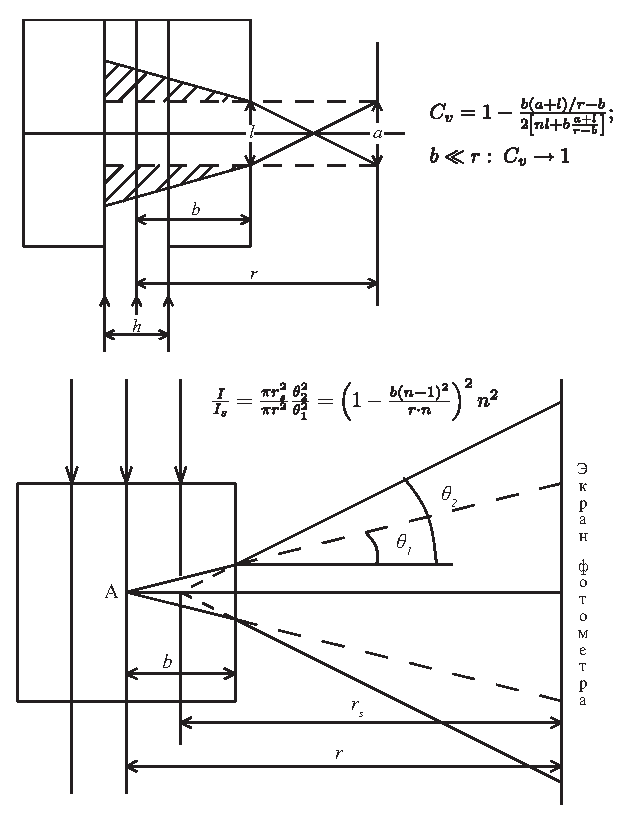
\includegraphics[scale=1.0]{Ris/ris_eps/ris5_2.eps}}}

\risp{2}{Методы Карра и Зимма}
\end{figure}

Отношение сигналов фотометра в этом случае
$$\ln{F_1\over F_2}=\tau\cdot l=10^{-2};\hskip 4mm {F_1\over
F_2}=1,03.$$
Т. е. два сигнала отличаются всего на 3\%. Для 1\% раствора
полистирола в бутаноне ($\tau_p=10^{-2}$ $\rm \hbox{см}^{-1}$),
использовалась кювета длиной $l=5$ см:
$$\ln{F_1\over F_2}=\tau\cdot l=5\cdot 10^{-2};\hskip 4mm
{F_1\over F_2}=1,05.$$
Здесь два сигнала отличаются на 5\%. Кроме этой оценки необходимо
отметить следующее. Как указывается в работе Карра и Зимма, поток
$F_2$ есть результат двух измерений, т. е. измерялись потоки
$F_1$, $F'_2$ и $F^0_2$, различие между которыми не может быть
определено таким приемником, как интегрирующий шар с
фотоэлементом:
$$\tau_{\rm \hbox{бутанона}}=0,5\cdot10^{-4}\ {\rm \hbox{см}^{-1}};\ \
\tau\cdot l=5\cdot10^{-4}\ {\rm \hbox{см}^{-1}}; \ \ \ln{F_1\over
F_2^0}=5\cdot10^{-4},$$
т. е. отношение сравниваемых потоков очень мало, а если оно
имеется, то обусловлено отнюдь не рассеянием растворителя, а
отражениями на стенках кюветы.

Авторы указывают, что три метода, предложенные ими для определеня
мутности растворов, независимы. Но это не совсем так. В первом
и втором методах используются для ослабления первичного пучка
одни и те же серые фильтры большой плотности, проградуированные
на установке с диффузором.

Для того, чтобы определить абсолютную рассеивающую способность
$\rm CCl_4$ и бензола, интенсивность света, рассеянного под углом
$90^{\circ}$ этими жидкостями, сравнивалась с интенсивностью
света, рассеянного растворами, мутность которых была определена
тремя указанными  выше способами. При этом, так как показатели
преломления жидкостей и растворов отличались, вновь вводились
поправки $C_n$ и $C_v$. Значения $R$, полученные авторами для
$\rm CCl_4$ и бензола, на 50\% превышали значения, полученные в
более ранних исследованиях (см. табл. 5.1).

Из сказанного выше можно сделать вывод, что все три метода
определения мутностей полистирола в растворах, используемых как
эталон для определения рассеивающей способности $\rm CCl_4$ и
бензола, не являются точными методами. Поэтому новые значения для
константы рассеяния, предложенные Карром и Зиммом, нельзя считать
более точными, как это утверждают авторы, обвиняя предыдущих
исследователей в том, что они не вводили поправок на преломление
рассеянных лучей.



%Исследования Вокулера

После работы Карра и Зимма, впервые опубликовавших высокие значения $R$, 
в лаборатории Кабанна в Сорбоне было выполнено подробное фотометрическое
исследование по измерению константы рассеяния фотографическим методом, 
опровергающее замечания Карра и Зимма о необходимости 
введения поправки $C_n$ в фотографических и визуальных измерениях.

В отличие от фотоэлектрических измерений, 
когда сравниваются световые потоки, фотографический метод измерения рассеивающей способности жидкостей заключается в сравнении яркости $b$ диафрагмы $\Delta$,
помещенной на пути рассеянного жидкостью под углом 90$^\circ$ пучка, с яркостью $b'$ диафрагмы $\Delta '$, ограничивающей пучок света, отраженный от эталонного диффузора, помещенного под углом 45$^\circ$ к направлению падающей освещенности, вместо рассеивающего объема. В качестве диффузора использовались фарфоровые пластинки, покрытые MgO или MgCO$^3$, с коэффициентом отражения $r=0,85\div0,95$ (источники Ламберта-Бера).

\begin{figure}[tbp]
\centerline{\hbox{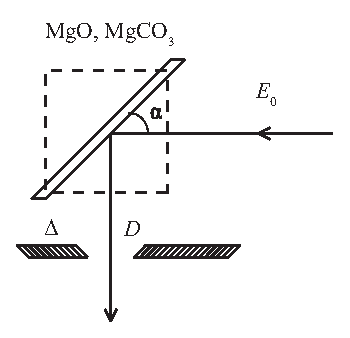
\includegraphics[scale=1.0]{Ris/ris_eps/ris5_3.eps}}}

\risp{3}{Фотографическое измерение рассеянной способности жидкостей. }
$S$ --- площадь диафрагмы $\Delta$, ограничивающей рассеивающий пучок; 
$D$ --- расстояние до диафрагмы от центра рассеивающего объема; 
$\alpha=45^{\circ}$; $r=0,85\div0,95$.
\end{figure}

Если $E_0$ --- освещенность падающего света, $E_0\cos i$ ---
световой поток, падающий на единицу поверхности диффузора (рис.
5.3), то:
$$b'={rE_0\cos i\over\pi},\noq$$
Если $D$
--- расстояние от диффузора до фотопластинки, $S$ --- площадь
диафрагмы, то
освещенность на поверхности фотопластинки
$$E_2={b'S\over D^2}={rE_0\cos i\over \pi}\cdot{S\over D^2}.\noq$$
Ослабляют падающий свет серыми фильтрами, так чтобы
$$E_1=kE_0=E_2.\noq$$
Определяют какую оптическую плотность $\delta=-\log k$ надо
ввести в первоначальный пучок, чтобы было выполнено соотношение
\eqn{12}. В этом и заключается предварительное эталонирование
диффузора.

Величину $\beta={r\cos\alpha\over\pi}={kD^2\over S}$ называют
фактором яркости диффузора. Константа рассеяния будет определена,
если измерены $\beta$, отношение яркостей рассеянного пучка и
диффузора, а также $h$ --- глубина рассеивающего объема.
Действительно, по определению
$$R={i_{90}\cdot r^2\over E_0\cdot V}={i_{90}\cdot r^2\over
S\cdot h\cdot E_0}={b\over E_0\cdot h}.\noq$$

Так как $b'=\beta E_0$, измеряют ${b'\over b=K}$, $\beta$ и $h$ --- глубину рассеивающего объема
$$ R = {\beta \over K\cdot h}. \noq$$

При измерениях с диффузором на пути падающего луча ставилась кювета с исследуемой жидкостью. Фокусировка изображения источника в центр кюветы рассеяния или на диффузор производилась при помощи подвижного конденсора, что позволио сохранять телесный угол, под которым лучи попадали в кювету. Эталонирование диффузора было произведено особо тщательно, --- угол $\alpha=45^{\circ}$, составляющий диффузором с направлением падающего луча, выдерживался при эталонировании и измерениях с точностью до $2'\div3'$.


Таким образом, яркость изображения диафрагмы $\Delta$ освещенной
диффузором, та же, независимо от того, будет ли диффузор помещен
в жидкость или будет находиться в воздухе, если производится
фокусировка источника в центр рассеивающей кюветы или на
плоскость диффузора при помощи подвижного конденсора.


%Исследования Пейро


Остановимся на фотографическом методе Пейро \  и фотоэлектрическом
методе измерения Блеккера, Баджера и Гильмана , чтобы
показать, что величина $R$ не зависит от методики измерений, если
не вводятся теоретически рассчитанные поправки.

В фотографических измерениях асболютной интенсивности света,
рассеянного безолом, произведенных в 1939 году Пейро, методика
выбрана так, что сходимость первоначального и рассеянного пучков
остается постоянной при сравнении света, рассеянного бензолом, с
яркостью первоначального пучка, т. е. тем самым, исключается
поправки на преломление лучей, выходящих из кюветы рассеяния
(рис. 5.6).

Пейро сравнивал яркость светового пучка, рассеянного бензолом
${\cal E}_1$ с яркостью истоника ${\cal E}_2$, создающего
освещенность $E$ в центре прямоугольной кюветы M в плоскости,
перпендикулярной к первоначальному пучку (см. рис. 5.6). Метод
измерения Пейро заключался в следующем. Сначала запаянная кювета
с хорошо очищенным бензолом помещалась в середину кюветы M,
заполненной бензолом.

\begin{figure}[tbp]
\centerline{\hbox{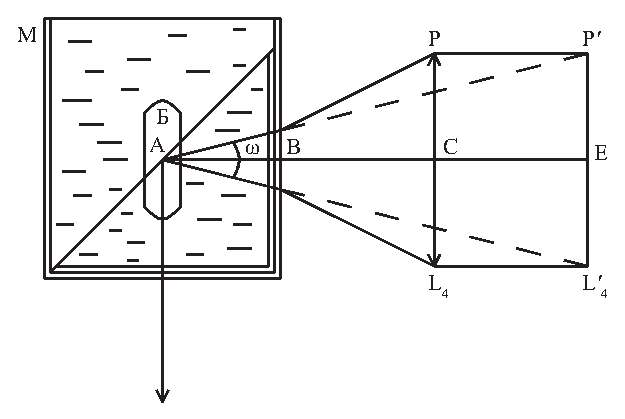
\includegraphics[scale=1.0]{Ris/ris_eps/ris5_4.eps}}}

\risp{4}{Установка Пейро.}
\end{figure}

По определению константы рассеяния $RI_0V=i_{90}\cdot r^2$,
откуда следует, что яркость рассеянного пучка
$${\cal E}_1={i_{90}\cdot r^2\over S}=REh,\noq$$
где $h$ --- освещенная глубина. Освещенность фотопластинки в этом
случае $$e_1=KREh.\noq$$
Затем бензол из кюветы выливался и призма полного внутреннего
отражения помещалась в кювету так, что линза L образовывала
изображение лампы на ее отражающей поверхности, составляющей угол
$45^{\circ}$ с первоначальным пучком. Призма занимала все
пространство между параллельными стенками кюветы. Для кюветы
подбиралось стекло, имеющее показатель преломления равный
показателю преломления бензола, поэтому сходимость
первоначального и рассеянного пучков остается той же, когда
переходит от измерений с бензолом к измерению яркости ${\cal
E}_2$ первоначального пучка, отраженного призмой.

Яркость источника ${\cal E}_2$ связана с нормальной освещенностью
$E$ следующим образом $E={\cal E}_2\omega$, где $\omega$ ---
телесный угол первоначального пучка в точке A. Освещенность
фотопластинки в этом случае
$$e_2=Kr{E\over\omega},\noq$$
где $r$ --- коэффициент ослабления яркости ${\cal E}_2$
нейтральными фильтрами. Почернения, пропорциональные $e_1$ и
$e_2$, получались при одинаковом времени экспозиции на одной и
той же фотопластинке. Константа рассеяния может быть получена,
если измерить ${e_1\over e_2},\ r,\ \omega$ и $h$:
$$R={e_1\over e_2}\cdot r\cdot {1\over\omega\cdot h}.\noq$$
Преломление в бензоле или равное ему преломление в стеклянной
призме учитывалось при определении телесного угла $\omega$
следующим образом (см. рис. 5.6):
$$\omega={S\over(AE)^2}={S\over(AB+BE)^2}={S\over(AB+BC\cdot
n)^2},\noq$$
где $S$ --- освещенная поверхность, выделяемая диафрагмой,
помещенной в плоскости P, против линзы L.

Для ослабления яркости
первоначального пучка использовалась система 3-х николей и
нейтральные поглощающие фильтры. Для $\lambda=4358$ \angst\ при
$t=20^{\circ}$C Пейро получил следующее значение
$$R=33,8\cdot10^{-6}\ {\rm \hbox{см}^{-1}}.$$
Ошибку опыта Пейро оценивает в 6-7\%.

Измерение отношения ${e_1\over e_2}$, входящего в \eqn{18},
выполнено в работе Пейро очень тщательно. Фактор $r$ определялся
несколькими способами; учитывались возможные потери при отражении
на границах стекло --- воздух воздух --- стекло. Глубину
рассеивающего объема Пейро также измерял несколько раз, помещая
фотопластинку в кювету, наполненную бензолом.

Блеккер, Баджер и Гильман, в свою очередь, предложили
фотоэлектрический метод определения $R$, в котором поправка на
преломление рассеянных лучей исключалась самими условиями опыта.

Источник, ртутная лампа, фокусируется на щель K, изображение
которой проектируется при помощи зеркала M и линз L в кювету
рассеяния. Исследуется рассеивающая способность $\rm CS_2$ для
$\lambda=5461$ \angst\ и $\lambda=4358$ \angst.
Интенсивность рассеянного света сравнивается с интенсивностью
падающего света при помощи двух фотоумножителей по методу
компенсации. Определение константы рассеяния $\rm CS_2$
разбивается на два этапа.

В первом опыте интенсивность падающего пучка сравнивается с
интенсивностью света, рассеянного от полированной фарфоровой
пластинки, подвешенной в кювете и погруженной в $CS_2$. Пластинка
подвешивалась так, что угол падения и угол рассеяния были оба
равны $45^{\circ}$.

Во втором опыте интенсивность света, рассеянного освещенным
объемом $\rm CS_2$ под углом $90^{\circ}$ к падающему пучку,
сравнивалась с рассеянием от фарфоровой пластинки. Падающий пучок
непараллельны и освещенность меняется от одной точки освещенного
объема к другой. Перемещая пластинку параллелльно самой себе в
направлении падающего пучка, выводится среднее эффективное
значение освещенности пластинки, исходя из кривой зависимости
светового потока в фотоумножителе от положения пластинки.
Эффективная интенсивность рассеяния пластинки, подвешенной в
кювете $\rm CS_2$, сравнивается с объемным рассеянием $\rm CS_2$,
при этом свет, рассеянный от пластинки и от освещенного объема
$\rm CS_2$, претерпевает одинаковое отражение и преломление на
стенках кюветы.

Рассеивающая способность $\rm CS_2$ достаточно велика, поэтому
сравнение интенсивности можно делать без применения нейтральных
фильтров большой плотности. Авторы получили следующие результаты
для рассеивающей способности $\rm CS_2$:
$$\hbox{для}\ \lambda=4358\angst,\ \ R=151\cdot10^{-6}\ {\rm
\hbox{см}^{-1}};$$
$$\hbox{для}\ \lambda=5461\angst,\ \ R=47,8\cdot10^{-6}\ {\rm
\hbox{см}^{-1}}.$$
Относительное рассеяние $\rm CS_2$ и бензола измерялось многими
авторами . Отношение ${R_{\rm CS_2}\over R_{\rm \hbox{бензола}}}=4,9$,
т. е. для бензола значения $R_{\rm \hbox{бензола}}$, полученные Блеккером,
Баджером и Гильманом, несомненно относятся к группе << низких>>\ значений.
$$R_{\rm \hbox{бензола}}=30\cdot10^{-6}\ {\rm \hbox{см}^{-1}}\ \ {\rm \hbox{для}}\ \
\lambda=4358\angst;$$
$$R_{\rm \hbox{бензола}}=10\cdot10^{-6}\ {\rm \hbox{см}^{-1}}\ \ {\rm \hbox{для}}\ \
\lambda=5461\angst.$$

Используя $\rm CS_2$ как стандарт, авторы определили рассеяние
растворов нитроцеллюлозы в ацетоне. Тщательная очистка растворов
от пыли производилась центрифугированием. Молекулярный вес,
полученный по методу светорассеяния, был определен как
$M_W=185000$.

Вискозиметрическим методом был получен молекулярный вес
$M_W=163000$. Методом светорассеяния определяется средневесовой
молекулярный вес $M_W$, который при наличии небольшой
дисперсности среды всегда несколько больше среднечисленного
молекулярного веса $M_h$, определяемого по методу измерения
вязкости растворов. Согласие между результатами двух методов
получилось хорошее, что, по мнению авторов, свидетельствует в
пользу правильных значений.

Однако, следует отметить, что получение правильного молекулярного
веса полимера по методу светорассеяния с применением жидкого
стандарта не может служить доказательством правильности
используемого абсолютного значения светорассеяния этого
стандарта.

Дело в том, что так называемый << правильный >>\ молекулярный
вес, с которым сравнивают молекулярный вес полимера, полученный
по методу светорассеяния, берется многими авторами из
относительных вискозиметрических измерений. При
вискозиметрических измерениях требуется дополнительная калибровка
с применением абсолютных методов (диффузионного,
криоскопического, осмометрического).


\subzag{Дискуссия}

Известные французские оптики Руссе и Лоше подробно рассмотрели фотоэлектрические и фотографические методики измерения $R$ и пришли к выводу, что имеющиеся расхождения не могут объясняться тем, что в фотографические измерения не вносится поправка $C_n$. По их мнению, при фотографическом методе измерения поправка $C_n$ вообще не должна вносится. Их вывод основан на следующем рассуждении. 

\vskip 0mm
\begin{figure}[tbp]

{\small
\tabp{1}{Коэффицтент $R$ бензола ($\lambda = 4358\angst$, $t = 20°C$)}
\begin{center}
 \begin{tabular}{| l | c | c | c |}
    \hline
    Авторы & Год & $R\cdot10^6$ & Метод \\ \hline
    Мартин и Лерман & 1922 & 32,8 & фотогр. \\ \hline
    Кабанн и Доор & 1927 & 28,5 & фотогр. \\ \hline
    Пейро & 1938 & 33,8 & фотогр. \\ \hline
    Баи & 1942 & 29,1 & ф.э. \\ \hline
    Блекер, Баджер, Гильман & 1949 & 29,8 & ф.э. \\ \hline
    Вокулёр & 1951 & 31,8 & фотогр. \\ \hline
    Штамм и Баттон & 1953 & 27,6 & ф.э. \\ \hline
    Харринд & 1953 & 28,0 & ф.э. \\ \hline
    Шапель, Торрель & 1955 & 31,0 & ф.э. \\ \hline
    Вукс и Рождественская & 1964 & 32,8 & ф.э. \\ \hline
    Рождественская и Горбачева& 1980 & 32,7 & ф.э. \\ \hline\hline
    Карр и Зимм & 1950 & 42,4 & ф.э. \\ \hline
    Брайс и др. & 1950 & 46,8 & ф.э. \\ \hline
    Марон и Лоу & 1954 & 57,0 & ф.э. \\ \hline
    Отт, Отт, Дезро & 1953 & 56,0 & ф.э. \\ \hline
    Кремен, Шапиро & 1954 & 46,3 & ф.э. \\ \hline
    Лент и др. & 1965 & 46,3 & ф.э. \\ \hline
    Денниген, Джекобс & 1970 & 50,02 & ф.э. \\ \hline\hline
    Кантов & 1956 & 43,4 & ф.э. \\ \hline
    Куму & 1960 & 44, & ф.э. \\ \hline
    Ландберг и др. & 1964 & 43,8 & ф.э. \\ \hline
    Кей и Хелвик & 1973 & 44,3 & ф.э. \\ \hline
    Кей и Мак-Даниэль & 1974 & 40,3 & ф.э. \\ \hline
    Пайк и др. & 1975 & 42,4 & ф.э. \\ \hline
  \end{tabular}
\end{center}
}
\end{figure}

Предположим, что рассеивающий объем ограничен диафрагмой $D$, помещенной в жидкость с показателем преломления $n$. Обозначим яркость изображения этой диафрагмы будет уже не $b$, а $b/n^2$, и освещенность фотографического изображения будет уменьшена в $n^2$ раз. Если теперь в рассеивающую жидкость погрузить магниевую пластинку (диффузор в работе Вокулера), то яркость диафрагмы в направлении ОА будет $b'/n^2$ и отношение освещенностей двух изображений будет по-прежнему равняться $b/b'$.

Однако в некоторых фотографических установках диффузор находится в кювете, не заполненной жидкостью. В этом случае источник при переходе от рассеивающей жидкости к диффузору не будет на нем сфокусирован. Для фокусировки изменяли положение конденсора и в результате юстировки телесный угол оказывался таким же, что  и в случае с рассеивающим объемом. В этом случае яркость магниевой пластинки уменьшается в $n^2$ раз, а яркость изображения диафрагмы, помещенной в воздух увеличивается в $n^2$ раз по сравнению с яркостью изображения диафрагмы $D$, освещенной магниевой пластинкой, погруженной в жидкость. Таким образом, и в этом случае результат остается прежним.

Анализ установок Вокулера, Пейро, приводит Руссе и Лоше к выводу, что к измерениям указанных выше авторов следует относиться как к безукоризненным фотографическим измерениям.

Подобный вывод был сделан J. Cabann в 1956 году при анализе фотографических измерений.

Несмотря на то, что Руссе и Лоше предприняли серьезный анализ экспериментальных фотографических и визуальных измерений и показали, что поправка $C_n$ вводиться не должна.

Необходимо было их выводы подтвердить независимым экспериментом исключающим возможность <<введения поправки>>\ на расходимость лучей при выходе из кюветы рассеяния, с другой стороны, учитывающей возможное собственное поглощение жидкостей вдали от полосы поглощения. М. Ф. Вуксом был предложен так называемый <<метод сравнения>>. В 1964 г. работа была выполнена Н. Б. Рождественской в Ленинградском Университете для трех жидкостей: $\rm Cl_4$, метилэтилкетона и бензола для двух длин волн 5461\angst\ и 4358\angst\ ртутного спектра были получены низкие значения константы рассеяния бензола, МЭК и четыреххлористого углерода.
Причем для каждой жидкости были применены и абсолютные измерения.

В методе сравнения и абсолютном методе вместо диффузора своего рода эталоном служил раствор полистирола в соответственной жидкости, раствор такой малой концентрации, что показатель преломления раствора отличался от показателя преломления жидкости в третьем знаке после запятой.

Следующие фундаментальные измерения были выполнены в Ленинградском Университете в 1979 году Н. Б. Рождественской и Е. Н. Горбачевой. Причиной, побудившей вновь обратиться к этой теме послужили два обстоятельства:

1. Появление лазеров.

2. Опубликованная Дж. Стоуном в 1972 году работа, где им было исследовано 27 прозрачных 
в видимой области жидкостей и показано, что в области далекой от полосы поглощения коэффициент 
собственного поглощения жидкостей $K$ такого же порядка, а для некоторых жидкостей много 
больше коэффициента мутности $\tau$. Дело в том, что столь малые собственное поглощение, 
сравнимое с мутностью $\tau$, меньше погрешности измерения любого спектрометра. Стоун сотоварищи 
производили измерения поместив кювету с прозрачной жидкостью в резонатор лазера. 
Из-за поглощения кювета нагревалась. Соответствующая градуировка с эталоном поглощения 
дала возможность определить собственное поглощение.
все работы по определению коэффициента мутности $\tau$. На спектрофотометре Бекмана, 
а затем расчет по формуле из $\tau$ величины коэффициента рассеяния некорректны, 
так как вместо используемой формулы $I=I_0e^{-\tau l}$ необходимо пользоваться формулой $I=I_0e^{-(\tau+K)l}$.

Из таблицы будет ясно, что значения для $R$ получились высокими, 
так как вместо $\tau$ в формуле $\tau={16\pi\over3}R$ на самом 
деле использовалось экспериментальное $(\tau+K)$.

Важность выполнения этой работы была очевидна и по следующим причинам. 
Экспериментальное определение коэффициента рассеяния чистых жидкостей 
важно для развития теории молекулярного рассеяния света. Точное значение 
коэффициента рассеяния необходимо для калибровки фотометров, используемых 
для измерения молекулярных весов полимеров. При изучении деполяризованного 
рассеяния неправильная калибровка фотометра даст некорректные результаты 
о характере развития ориентационных парных корреляций между анизотропными
молекулами. Наконец, значение коэффициента рассеяния используется о формулах 
молекулярного и двойного лучепреломления и деполяризованного рассеяния света.


\markright{\hfill\small Метод Вукса-Рождественской
в жидкости\hfill}{}

\subzag{Метод Вукса-Рождественской для определения коэффициента рассеяния в жидкости}

\markright{\hfill\small Метод Вукса-Рождественской
в жидкости\hfill}{}

\vskip 2mm
Рассеивающая способность жидкостей характеризуется величиной
коэффициента рассеяния, не зависящей от условий эксперимента
$$R={I_{90}r^2\over I_0V}, \noq$$
где $I_0$ --- интенсивность падающего света, $I_90$ ---
интенсивность света, рассеянного под углом $90^{\circ}$, $V$ ---
рассеивающий объем, $r$ --- расстояние от рассеивающего объема до
точки наблюдения. 

Для жидкостей, сдержащих оптически анизотропные молекулы термодинамическая теория приводит к формуле

$$R={\pi^2\over2\lambda^4}\left[kT\beta_S\left(\rho{\partial\varepsilon\over\partial
\rho}\right)^2_S+{\sigma^2kT^2\over\rho C_p}\left({1\over\rho}{\partial\varepsilon\over
\partial T}\right)^2_p\right]\cdot{6+6\Delta\over6-7\Delta}, \noq$$

Используя соотношение Ландау-Плачека для $J_{is}$ и $J_{ad}$ интенсивностей рассеяния

$${R_{is}\over R_{ad}} = {\left( {1\over\sigma}{\partial\varepsilon\over\partial T}\right)^2_p \sigma^2 T \over \left(\rho{\partial\varepsilon\over\partial\rho}\right)^2_s\rho\beta_s }, \noq $$

Из (3) можно получить:

$$ R = {2\pi^2\over\lambda^4} k T^2 n^2 ({\partial n\over\partial \rho})^2_p\cdot {1\over\rho C_p}\left(1+{R_{ad}\over R_{is}}\right){6+6\Delta\over 6-7\Delta}, \noq $$

Формула Эйнштейна:
$$ R={\pi^2\over 2\lambda^4}kT\beta_T - (\rho{\partial\varepsilon\over \partial\rho})^2_T. \noq $$
Экспериментальные измерения с помощью этой формулы затруднительны и неточны. Приближенные формулы дают разные результаты.
Погрешности составляют порядка 30~\%. 

Только формула М.~В.~Вукса дает хорошее согласие с экспериментальными данными (порядка 2$\div$3~\%):
$$ R = {\pi^2\over2\lambda^4}kT\left(\beta_s+{\sigma^2\over\rho C_p}\right)(n^2-1)^2\left({3n^2\over2n^2+1}\right){6+6\Delta\over6-7\Delta}. \noq $$

Определение молекулярного веса полимеров по методу Дебая (рассеяние света) связана с рассеянием на флуктуации концентрации полимера в растворе.
Для разбавленного раствора полимера:

$$ R_k = {2\pi^2 n^2\over\lambda^4N_a}\left({\partial n\over\partial c}\right)^2_{\hbox{флукт.}}c\cdot M, \noq $$
где $M$ --- молекулярный вес, $c$ --- концентрация полимера. В статьях, опубликованных до 1970 года величина $({\partial n\over\partial c})_{\hbox{флукт.}}$ 
идентифицировалась с величиной ${(n-n_s)\over c}$, где $n_s$ --- показатель преломления растворителя; n --- показатель преломления раствора.

В.~М.~Вукс получил формулу:
$$ \left({\partial n\over\partial c}\right)^2_{\hbox{флукт.}} = {(n\cdot n_s)^2\over c^2}\left({3n^2\over2n+1}\cdot{3\over n^2+2}\right)^2. \noq $$

Для растворов в бензоле, при $\lambda=4358$\angst, $n=1,5209$ эти величины отличаются на 26 \%.
$$ \left({\partial n\over\partial c}\right)^2_{\hbox{флукт.}} = \left({n-n_s\over c}\right)^2\cdot 0,74, $$
поэтому если использовать точную формулу \eqn{7} для получения правильных молекулярных весов необходимо
пользоваться <<низкими>> значениями для калибровки установки. Только в этом случае полученные методом рассеяния света значения $M$
будут соответствовать молекулярным весам, полученным по методам седиментации, осмометрии и др.

М. Ф. Вуксом был предложен метод определения $R$, не содержащий каких-либо замечаний в смысле необходимости введения поправок на расходимость лучей при выходе из кюветы
рассеяния. Еще раз вспомним <<предмет дискуссии>>, две причины возникновения результатов с высокими и низкими значениями.

1. Неточность  поправок для преломления рассеянных лучей при выходе из кюветы, --- $C_n$.

2. Факт наличия собственного поглощения в прозрачных жидкостях вдали от полосы поглощения, сравнимого по величине с ослаблением вследствие рассеяния.

Предложенный метод исключает вышеуказанные поправки. В процессе измерения сравниваются два световых потока $B_{\hbox{ж}}$ и $B_{\hbox{р}}$, проходящие
через чистую жидкость и слабый раствор полимера в этой жидкости (низкий молекулярный вес, $d << \lambda$, т.~е. рэлеевское рассеяние.
$$ \tau_p - \tau_{hbox{ж}} = ({1\over l})\ln{B_{hbox{ж}}\over B_p} = b \noq $$

Сравниваются интенсивности света, рассеянного под углом 90° от чистой жидкости и раствора.
$$ {I^{90}_{p}\over I^{90}_{hbox{ж}}} = {R_{vр}\over R_{v\hbox{ж}}}\equiv
a' \noq $$
где $R_v$ --- фактор рассеяния для вертикально-поляризованного света, связан с $\tau$ как 
$$ R_v = \tau {3\over8\pi} {1+\Delta_v\over 1+2\Delta_v}, \noq$$
где $\Delta_v$ - коэффициент деполяризации вертикально поляризованного падающего света. 

Сравнивая \eqn{27} и \eqn{30}, получим
$$ \tau_{\hbox{ж}} = {b\over a-1} \noq $$

После некоторых преобразований, получаем следующую формулу для естественного (неполяризованного) света:

$$ R_{\hbox{ж}} = {3\over 16\pi} \tau_{\hbox{ж}} {1+3\Delta_{v_{\hbox{ж}}}\over
1+2\Delta_{v_{\hbox{ж}}}} \noq $$

Таким образом мы имеем два способа получения абсолютной рассеивающей способности чистых жидкостей:

Формула \eqn{31} --- метод сравнения;

Формула \eqn{22} --- метод измерения высокой разрешающей силы тонкой структуры
линий рассеяния.

% ****** Begin of experiment description ******


Схема установки приведена на рисунке. Свет от источника попадает
на светоделитель $П_1$ (стеклянная плоскопараллельная пластинка)
и делится на 3 пучка. Модулятором служит диск с тремя вырезанными
секторами, в каждый момент времени пропускающий либо 1-й, либо
2-й и 3-й пучки. Свет модулируется с частотой 140 Гц.
Преимущество выбранного модулятора (прерывателя) $M$ перед часто
используемым зеркальным заключается в том, что не требуется
точная установка плоскости вращения. 1-й пучок проходит через
кювету, 2-й делится на 2 пучка сравнения ($2а$ и $2б$) для
проходящего и рассеянного света.

В сравнительном эксперименте для ослабления потоков сравнения
используются одни и те же нейтральные светофильтры $F_1$ и $F_2$,
и поэтому не было необходимости их дополнительно градуировать.
Измерения проводятся с помощью системы из трех поляризаторов
(призмы Франка --- Риттера 10 $\times$ 10 мм) $P_1$, $P_2$,
$P_3$. $P_1$ и $P_3$ установлены неподвижно и поляризуют свет в
вертикальном направлении. Призма $P_2$ может вращаться. Угол
поворота определяется с по шкале теодолита с нониусом с точностью
30$''$. После прохождения системы трех призм интенсивность
светового потока пропорциональна $I\sim\sin^{-4}\varphi$, где
$\varphi$ --- угол поворота призмы $P_2$, отсчитываемый от
положения, при котором $P_2$ скрещена с призмами $P_1$ и $P_3$.

\begin{center}
\begin{figure}[t]
\centerline{\hbox{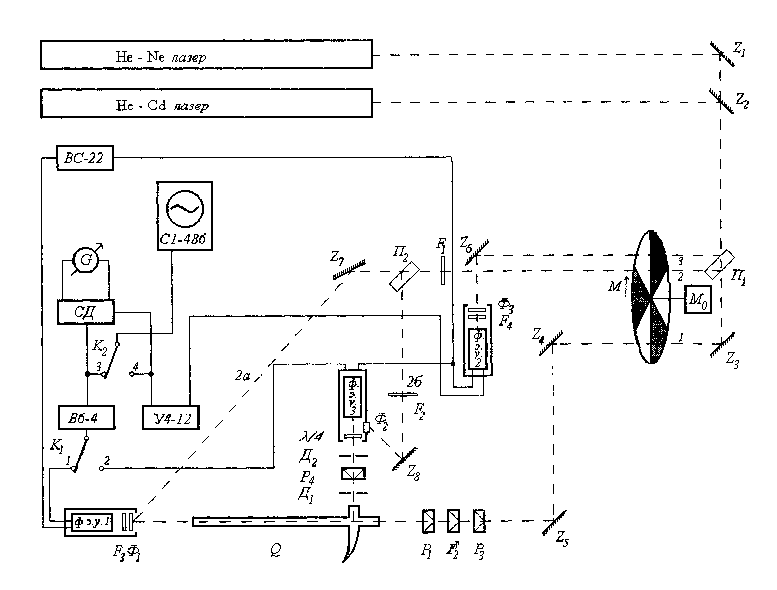
\includegraphics[scale=0.8]{Ris/ris_eps/ris5_3d.eps}}}

\risp{3a}{Схема установки для определения }
{\ris 
коэффииента
рассеяния жидкостей абсолютным методом 
$Z_1\div Z_8$ ---
поворотные зеркала, $F_1\div F_4$ --- нейтральные светофильтры,
$Ф_1$, $Ф_2$, 
$Ф_3$ --- рассеиватели, $П_1,$ $П_2$ --- стеклянные
плоскопараллельные пластинки,
$М$ --- модулятор, $P_1\div P_4$
--- поляризационные призмы Франка --- Риттера, $Д_1$, $Д_2$ ---
диафрагмы, 
$\lambda/4$ --- слюдяная пластинка, B6-4 ---
селективный усилитель,
У4-12 --- усилитель-ограничитель опорного
сигнала, $G$ --- гальванометр, 
С1-48Б --- осциллограф, $К_1$,
$К_2$ --- переключатели, $Q$ --- кювета, $СД$ --- синхронный
детектор}
\vskip -8mm
\end{figure}
\end{center}
%\hbox{\vbox to 13 true cm{\special{em:graph ris5_3d.bmp}}}

Приемниками излучения служат фотоумножители ФЭУ-51,
обеспечивающие высокие значения отношения с./ш. Использование
высокочувствительных ф.э.у. вызвано необходимостью регистрации
слабых световых потоков. Были отобраны ф.э.у. с возможно более
близкими характеристиками. Фотоумножитель, регистрирующий
проходящий световой поток и поток сравнения $(2а)$, защищен
плотными нейтральными светофильтрами $F_3$ и рассеивателем $Ф_1$
для более равномерного освещения фотокатода. Сигнал, снимаемый с
1-го ф.э.у., $\sim0,5$ В. Апертура рассеянного света
ограничивается диафрагмами $Д_1$ и $Д_2$. Пластинка $\lambda/4$
устраняет влияние возможной различной чувствительностью
фотоумножителя к горизонтально и вертикально поляризованному
свету. Сигнал, снимаемый со 2-го ф.э.у., $\sim3$ мВ. Призма
Франка --- Риттера $P_4$ служит для измерения степени
деполяризации. Поток сравнения $(2б)$ поступает на 2-й ф.э.у.
через фторопластовый рассеиватель $Ф_2$, вставленный в отверстие
кожуха фотоумножителя для равномерного освещения фотокатода и для
того, чтобы незначительные перемещения светового пятна на
фотокатоде не влияли на результат измерения. Третий пучок через
плотные нейтральные фильтры $F_4$ и рассеиватель $Ф_3$ попадает
на 3-й ф.э.у.

Питание фотоумножителей --- от стабилизированного выпрямителя
BC-22. Измерения отношения проходящего светового потока к потоку
сравнения и потока, рассеянного под углом $90^{\circ}$ к потоку
сравнения, совершаются поочередно. В положении {\it 1}
переключателя $K_1$ происходит измерение отношения проходящего
через кювету с жидкостью или раствором светового потока к потоку
сравнения, то есть сигнал с 1-го ф.э.у. поступает на селективный
усилитель В6-4, настроенный на частоту 140 Гц (полоса пропускания
15 Гц). Измерение отношения рассеянного под углом $90^{\circ}$
светового потока к потоку сравнения произвоится при положении
{\it 2} переключателя $K_1$. Контроль за выравниванием
интенсивности измеряемых потоков и потоков сравнения
осуществляется с помощью осциллографа С1-48Б (положение {\it 3}
переключателя $K_2$), собранного по двухполупериодной  релейной
схеме. Опорный сигнал прямоугольной формы формируется
усилителем-ограничителем, на который поступает сигнал с 3-го
ф.э.у. В качестве усилителя-ограничителя используется стандартный
измерительный усилитель У4-12. Равенство нулю постоянной
составляющей на выходе синхронного детектора регистрируется
гальванометром магнитоэлектрической системы М91.

\centerline{\hbox{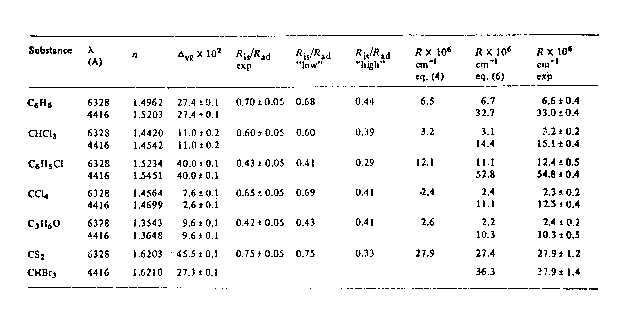
\includegraphics[scale=1.2]{Ris/ris_eps/table_opt_comm.eps}}}

Многократные измерения коэффициента рассеяния бензола дали
значения (31,1 $\pm$ 0,4)$10^{-6}$ $\rm \hbox{см}^{-1}$ для
$\lambda=$4400 \angst\ и (6,2 $\pm$ 0,8)$10^{-6}$ $\rm \hbox{см}^{-1}$ для
$\lambda=$6328 \angst\ при $t=23^{\circ}$C, что хорошо
согласуется с ранее измеренными значениями $R$ для $\lambda=4358$
\angst ($34,0\cdot10^{-6}$ $\rm \hbox{см}^{-1}$) и $\lambda=5461$ \angst
($12,6\cdot10^{-6}$ $\rm \hbox{см}^{-1}$) с учетом зависимости
коэффициента рассеяния от длины волны.

% ***** end of experiment description ****


В таблице приведены результаты измерений констант рассеяния $R$ для семи 
жидкостей при $T = 25°$~C и для двух длин волн: 
$\lambda = 6328 \angst$ (He-Ne лазер) и $\lambda = 4416 \angst$ (He-Cd лазер). 
Степень деполяризации $\Delta_{\hbox{ж}}$; отношение Ландау-Плачека 
$R_{is}/R_{ad}$ --- определенное по спектрам тонкой структуры (5 столбец). 
В 6 столбце $R_{is}/R_{ad}$, расчитанное из <<низкого>> значения $R$. 
В 7 столбце значение $R_{is}/R_{ad}$, рассчитанное из высокого значения $R$. 
Далее $R$ рассчитанное из уравнения \eqn{22}, используя значения $R_{is}/R_{ad}$,
полученные из эксперимента. Предпоследний столбец --- расчет по формуле \eqn{24}.
Последний столбец --- экспериментально определенные значения $R$ по методу М.~Ф.~Вукса --- абсолютные измерения для двух длин волн, независимо для каждой из семи жидкостей.

Значения $R_{is}/R_{ad}$, рассчитанные из <<низких>>\ значений $R$ находятся в хорошем согласии 
с экспериментальными значениями $R_{is}/R_{ad}$, и не согласуются со значениями, 
рассчитанными из <<высоких>>\ значений.

Точное знание величины $R$ необходимо для развития теории молекулярного рассеяния в жидкостях. 
Знание $R$ необходимо для калибровки фотометра для измерений 
по определению молекулярных весов полимеров по методу Дебая. 
%stop


